\section{Reasoning vs. Pattern‑Matching in LLMs}
\begin{frame}{}
    \LARGE Reasoning vs. Pattern‑Matching in LLMs
\end{frame}

\begin{frame}[allowframebreaks]{Reasoning vs. Pattern‑Matching in LLMs}
    \begin{itemize}
        \item \textbf{Pattern-Matching Models}
        \begin{itemize}
            \item \textbf{How it works:} LLMs are trained on vast amount of text data to learn statistical associations between words and phrases.
            \item \textbf{Characteristics:}
            \begin{itemize}
                \item Generate text based on learned patterns without deeper understanding.
                \item Often produce fluent and coherent text.
                \item May struggle with complex reasoning tasks or multi-step logic.
            \end{itemize}
            \item \textbf{Example:} Given the prompt ``The capital of France is'', the model outputs ``Paris'' by recalling frequent patterns in the training data.
            \item \textbf{Limitations:}
            \begin{itemize}
                \item May produce plausible-sounding but incorrect answers if the pattern is misleading.
                \item Struggles with tasks that require connecting multiple facts or reasoning through steps.
            \end{itemize}
        \end{itemize}
    \framebreak
        \item \textbf{Reasoning-Focused Models}
        \begin{itemize}
            \item \textbf{How it works:} LRMs extend LLMs by incorporating structured reasoning techniques.
            \item \textbf{Characteristics:}
            \begin{itemize}
                \item Generate structured intermediate steps to arrive at conclusions.
                \item Use multi-hop inference to connect information across several statements or facts.
                \item Can break down complex problems into smaller, logical steps.
            \end{itemize}
            \item \textbf{Example:} To answer ``If Alice has 3 apples and buys 2 more, how many does she have?'', the model first adds 3 and 2, then states the answer.
            \item \textbf{Benefits:}
            \begin{itemize}
                \item Provides explanations or shows their thought process, making answers more transparent.
                \item Better at tasks that require logic, calculation, or combining information from different sources.
            \end{itemize}
        \end{itemize}
    \framebreak
        \item \textbf{Examples}
        \begin{itemize}
            \setlength{\itemsep}{2em} % Adjust item spacing
            \item ``Which is heavier: a kilogram of feathers or a kilogram of iron?'' \\[1em]
            A pattern-matching model may be misled by the association of ``iron'' with heaviness. \\[1em]
            A reasoning model will recognize that both weigh the same.
            \item In logic puzzles, pattern-based models tend to contradict earlier premises \\[1em]
            Reasoning-aware models (e.g., using Chain-of-Thought prompting) remain consistent and logical.
        \end{itemize}
    \framebreak
        \begin{figure}[h]
            \centering
            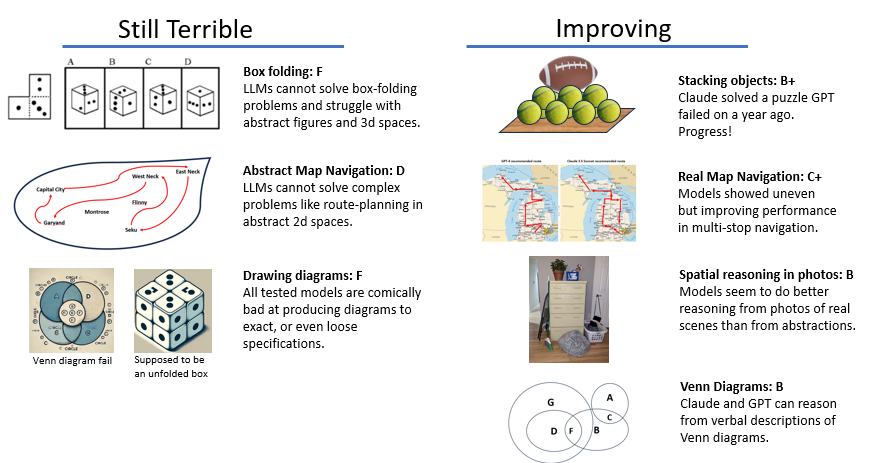
\includegraphics[height=0.8\textheight,width=\textwidth,keepaspectratio]{images/lrm+moe/lm-spatial-reasoning.png}
        \end{figure}
    \framebreak
        \item \textbf{Empirical Separation: When Does Reasoning Matter?}
        \begin{itemize}
            \item On simple factual questions, both model types may perform well.
            \item For challenging tasks like GSM8K (grade-school math), symbolic reasoning, or logic puzzles, pattern-matching alone is not enough.
            \item Success on these benchmarks improves dramatically when models are prompted to reason step by step (e.g., using Chain-of-Thought prompting).
            \item \textit{Example:} In multi-step math problems, models that show their work (reasoning-focused) achieve much higher accuracy than those that just guess the answer.
            \item This highlights the need for explicit reasoning capabilities in advanced language models.
        \end{itemize}
    \end{itemize}
\end{frame}